%%%%%%%%%%%%
% Preamble %
%%%%%%%%%%%%
% set document type, section numbering, and biblography style
\documentclass[twoside, 12pt]{article}
\usepackage{fullpage, graphicx, mathtools, gensymb, mhchem, siunitx, xr, xcolor, float}
\usepackage[english]{babel}
\usepackage[labelfont=bf]{caption} 
\usepackage[super,sort&compress,comma,round]{natbib}

% set fonts
\renewcommand*\familydefault{\sfdefault}
%\usepackage{sansmathfonts}

% highlight Chris's changes and comments
\newcommand{\car}[1]{\color{blue}#1\color{black}}
\newcommand{\comment}[1]{\color{red}#1\color{black}}

% other new commands
\newcommand{\velst}{$v_\mathrm{elst}$}
\newcommand{\rb}{$\rho_\mathrm{B}$}
% set the title material
\title{\vspace{-1em}\textbf{Excitation Shift of Retinal in channelrhodopsin}}
\author{\normalsize Nico and Cris}
\date{\normalsize \today}

%%%%%%%%%%%%%
% Main Text %
%%%%%%%%%%%%%
\begin{document}
\maketitle
%\tableofcontents
%%%%%%%%%%%%%%%%
% Introduction %
%%%%%%%%%%%%%%%%
\section{Overview}

The goal of this project is to assess the approximation:
\begin{equation}
\langle \hat{O}[\rho]\rangle \approx \hat{O}[\langle \rho \rangle]
\end{equation}
for the description of an average environment, applied to the first excitation ($\pi\to\pi^*$) of the embedded retinal in the Channelrhodopsin protein. See figure \ref{fig:mos} for the molecular orbitals involved in this excitation.\\
However, a particular challenge of this project is the fact that the solute, in this case retinal, is not rigid. In fact, the structure change of the retinal along the trajectory has a considerably important effect on the first excitation energy, generating shifts as large as approx. 0.7 eV, even larger than the environment effect, which is around 0.3-0.4eV \cite{Suliman2020}.

%%%%%%%%%%%%%%%%%%%%%%%%%%%%%%%%%
% Orbitals
\begin{figure}[H]
\centering
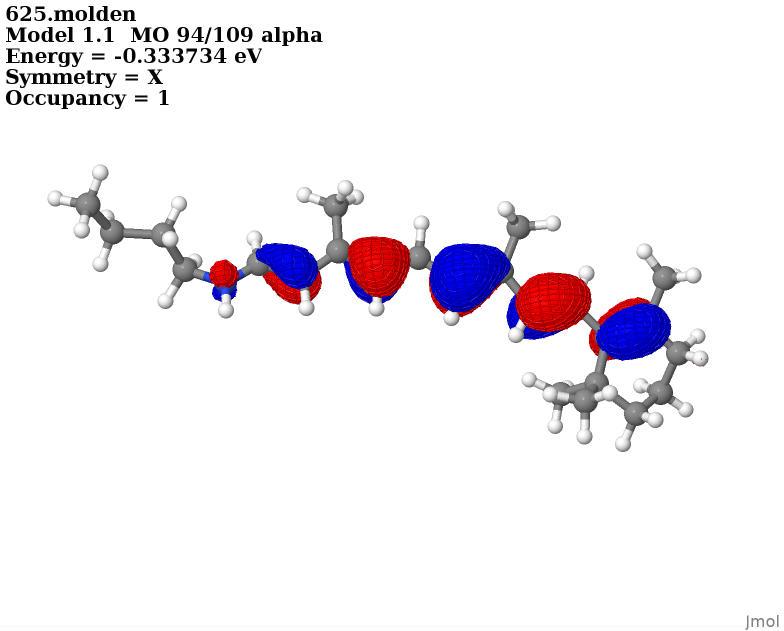
\includegraphics[width=8cm]{./figures/625_94.jpg}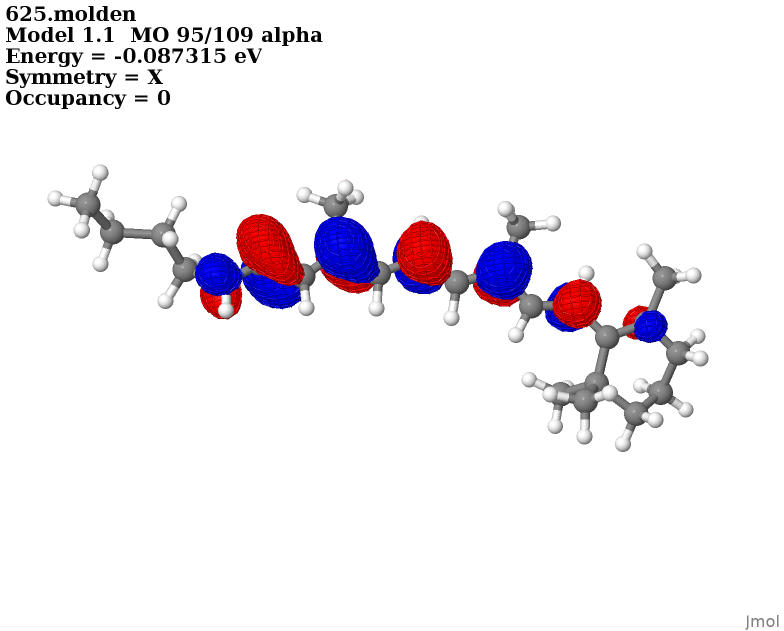
\includegraphics[width=8cm]{./figures/625_95.jpg}
\caption{Frontier molecular orbitals of retinal, HOMO the top, and LUMO at the bottom, where the excitation happens. The isosurface cutoff used was 0.03 a.u.} 
\label{fig:mos}
\end{figure}
%%%%%%%%%%%%%%%%%%%%%%%%%%%%%%%%%


%%%%%%%%%%%
% Results %
%%%%%%%%%%%
\section{Initial Results}

%%%%%%%%%%%%%%%%%%%%%
% Isolated retinal  %
%%%%%%%%%%%%%%%%%%%%%
\subsection{Spectrum of retinal}
\label{sec:init_results}
A MD trajectory of 750 frames, where all the atoms around the retinal in a radius of 12 \AA. where taken into account in different ways: the atoms within 5 \AA.  are computed as superposed electron densities, and the rest as point-charges.
The first excitation energy of the isolated retinal and the embedded retinal were computed with ADC(1)/cc-pvdz.
The corresponding spectrum is shown in \ref{fig:spec}. The averages are at 3.044 eV, for the embedded retinal at 3.418 eV, giving a shift of 0.374 eV.
As shown in figure \ref{fig:spec}, the peaks lay in 3.04 eV for the iso and 3.43 eV for embedded system. Using pointier Gaussian function (multiplying the exponential to 25.0) we obtain figure \ref{fig:spec_pt} the maximum are at 3.01 eV and 3.40 respectively [shift of 0.39 eV].


%%%%%%%%%%%%%%%%%%%%%%%%%%%%%%%%%
% Spectrum
\begin{figure}[H]
\centering
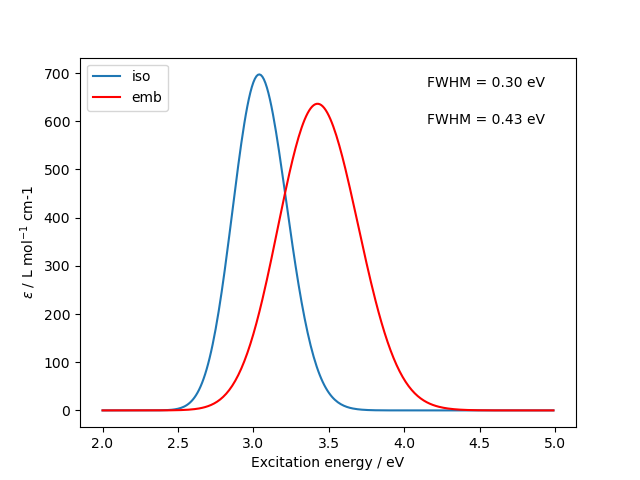
\includegraphics[width=10cm]{./figures/both_spectrum.png}
\caption{Spectrum of retinal from 750 frames MD trajectory.} 
\label{fig:spec}
\end{figure}
%%%%%%%%%%%%%%%%%%%%%%%%%%%%%%%%%

%%%%%%%%%%%%%%%%%%%%%%%%%%%%%%%%%
% Spectrum
\begin{figure}[H]
\centering
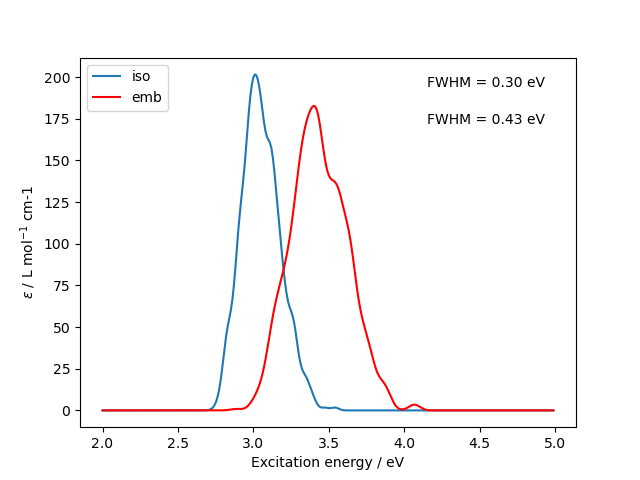
\includegraphics[width=10cm]{./figures/both_spectrum_pointy.png}
\caption{Spectrum of retinal from 750 frames MD trajectory.} 
\label{fig:spec_pt}
\end{figure}
%%%%%%%%%%%%%%%%%%%%%%%%%%%%%%%%%

When plotting:
\begin{equation}
a(x) = \sum_i \frac{f_i}{\sum_j f_j} \exp\left(-\frac{1}{2}\,c_{exp}\left(\frac{x - \epsilon_i}{\sigma}\right)^{2}\right) 
\label{eq:lineshape}
\end{equation}
where ${f_i}$ are the oscillator strengths, $\epsilon_i$ are excitation energies in eV, and $c_{exp}$ is a constant that determines the sharpness of the Gaussian functions used, the peaks seem to appear at 3.17 eV and 3.56 eV for the isolated and the embedded retinal respectively. The solvatochromic shift is 0.39 eV.


%%%%%%%%%%%%%%%%%%%%%%%%%%%%%%%%%
% Spectrum
\begin{figure}[H]
\centering
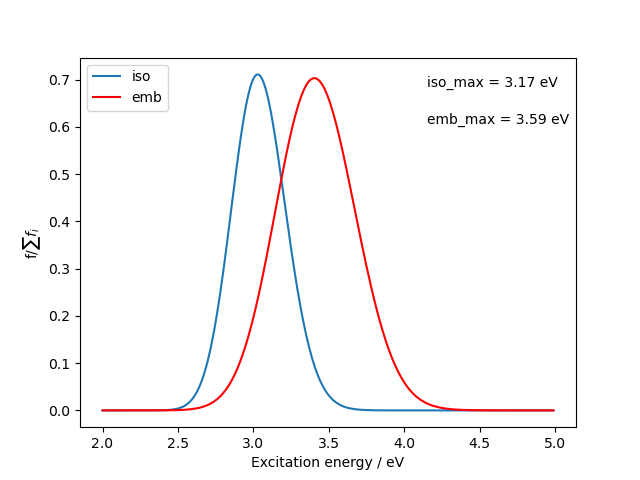
\includegraphics[width=9cm]{./figures/both_lineshape_broad.png}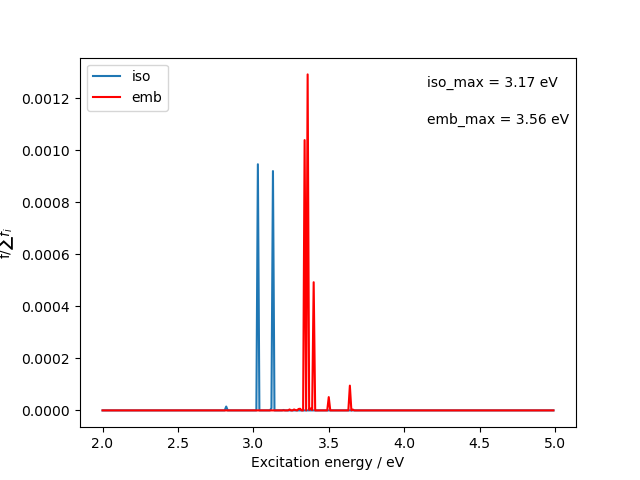
\includegraphics[width=9cm]{./figures/both_lineshape_sharp.png}
\caption{Lineshapes from 750 frames MD trajectory, following equation \ref{eq:lineshape}. Top: $c_{exp}$=1.0, bottom $c_{exp}$=$10^{8}$. } 
\label{fig:lineshape}
\end{figure}
%%%%%%%%%%%%%%%%%%%%%%%%%%%%%%%%%



\subsection{Averaging methods}
Within the fdeta package, the ic\_averager submodule allows averaging in internal coordinates.
Some issues can arise, and one or more methods are available to tackle them.
\begin{itemize}
 \item \textbf{quasilinear dihedrals}: dihedrals close to 180° appear to switch continuously between ~180° and ~-180°, resulting in an average of ~0°. Solutions
\begin{itemize}
 \item this can be detected via observing both the -180°-180° range and the 0°-360° range, and always average in the one with the lower standard deviation. Values averaged in the 0°-360° need to be converted again to the -180°-180°
 \item this could be fixed averaging angular displacement instead of the angle. This would be more computationally expansive, and is not implemented yet.
\end{itemize}
\item \textbf{freely rotating groups}: methyls, hydroxy, and several other groups cannot be averaged directly, as one would obtain a very similar value of ~0° for all the rotating dihedrals. Detection:
\begin{itemize}
 \item such angles can be detected with a threshold for the standard deviation in the optimal range (either 0°-360° or -180°-180°)
 \item this could be fixed following angular displacement instead of the angle. Continuously growing angular displacement would characterise freely rotating groups. This would be more computationally expansive, and is not implemented yet.
 \end{itemize}
Solutions:
\begin{itemize}
 \item the dihedral values of the first frame can be taken
 \item (slightly) preferential positions can be detected via cluster recognition in the distribution
\end{itemize}
\item \textbf{conformer-related groups}: hindered rotation (i.e. with a strong preferential position or set thereof), or conformers (e.g. cycloalkanes) can be averaged directly, but generally lead to a higher energy structure, more similar to the transition state between the more stable preferred structured. Detection:
\begin{itemize}
 \item such angles can be detected with a threshold for the standard deviation in the optimal range (either 0°-360° or -180°-180°)
 \item this could be fixed following angular displacement instead of the angle. Quasi-constant regions of angular displacement separated by jumps would characterise conformer-related groups. This would be more computationally expansive, and is not implemented yet.
 \end{itemize}
 Solutions:
\begin{itemize}
 \item the dihedral values of the first frame can be taken 
 \item preferential positions can be detected via cluster recognition in the distribution
\end{itemize}

\end{itemize}

Presently, the averaging within a recognised preferential position is done indepentently of the other variables. For instance, specific dihedral groups are averaged only in a specific set of frames, corresponding to a conformer, but angles and bond lenghts are averaged throughout the trajectory. This is an approximation and may be corrected in the future.

\subsection{Averaging retinal}
The aforementioned methods have been tested on the LYR fragment throughout the trajectory.
The files are named [method1]-[method2]-[descriptor], where \textit{method1} is the method used for ``oscillating'' or conformer-related groups, \textit{method2} is the method for rotating groups, \textit{descriptor} is an optional additional descriptor.

During the analysis of the obtained structures, an interesting feature was noticed: dihedral 49 ``oscillates'' between two conformers, but since the change in value is very small, this cannot be detected (lower standard deviation of \~20, comparable to standard angles). This is because C\-49 is in the alkyl cycle, but in $\beta$ to a double bond.

Even for humans, detection of these two conformers is possible when looking at the time evolution (see Fig. \ref{dih49evo}), but not obvious when the time information is removed (see Fig \ref{dih49distrib}).

%%%%%%%%%%%%%%%%%%%%%%%%%%%%%%%%%
% Time evolution
\begin{figure}[H]
\centering
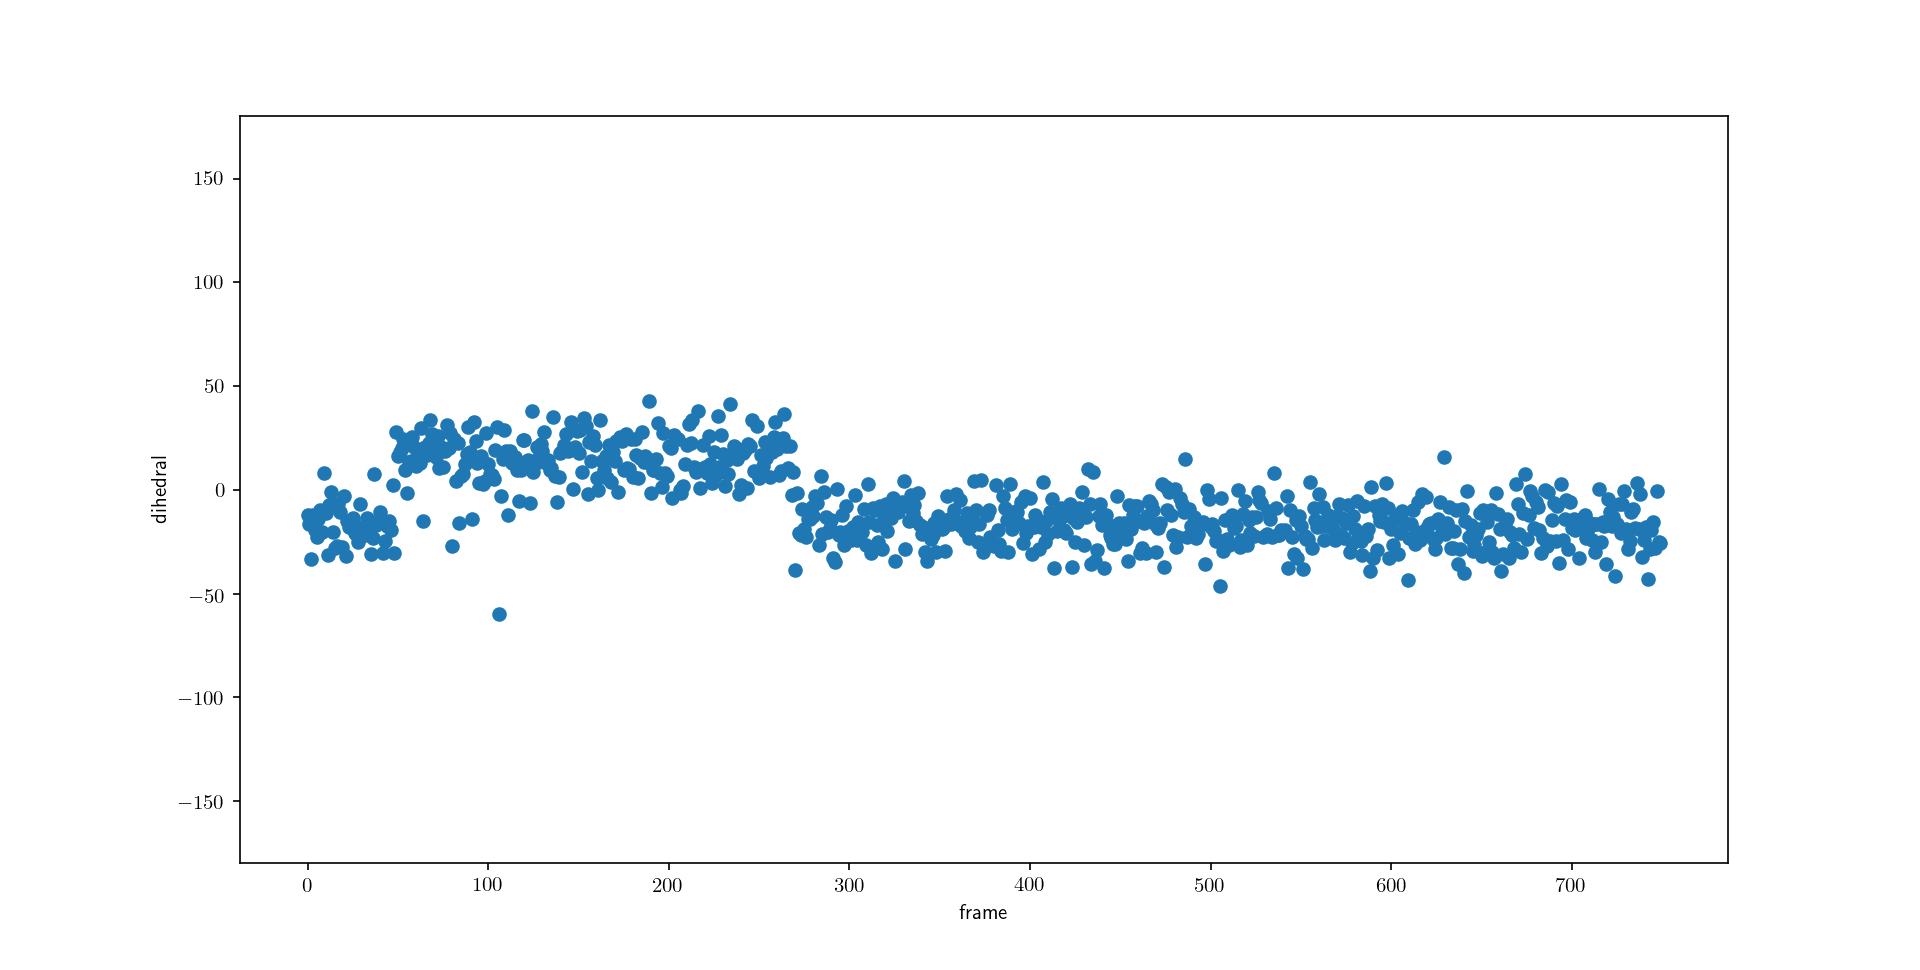
\includegraphics[width=0.95\textwidth]{./figures/dih49_evo.png}
\caption{Time evolution of dihedral 49.} 
\label{fig:dih49evo}
\end{figure}
%%%%%%%%%%%%%%%%%%%%%%%%%%%%%%%%%

%%%%%%%%%%%%%%%%%%%%%%%%%%%%%%%%%
% Time evolution
\begin{figure}[H]
\centering
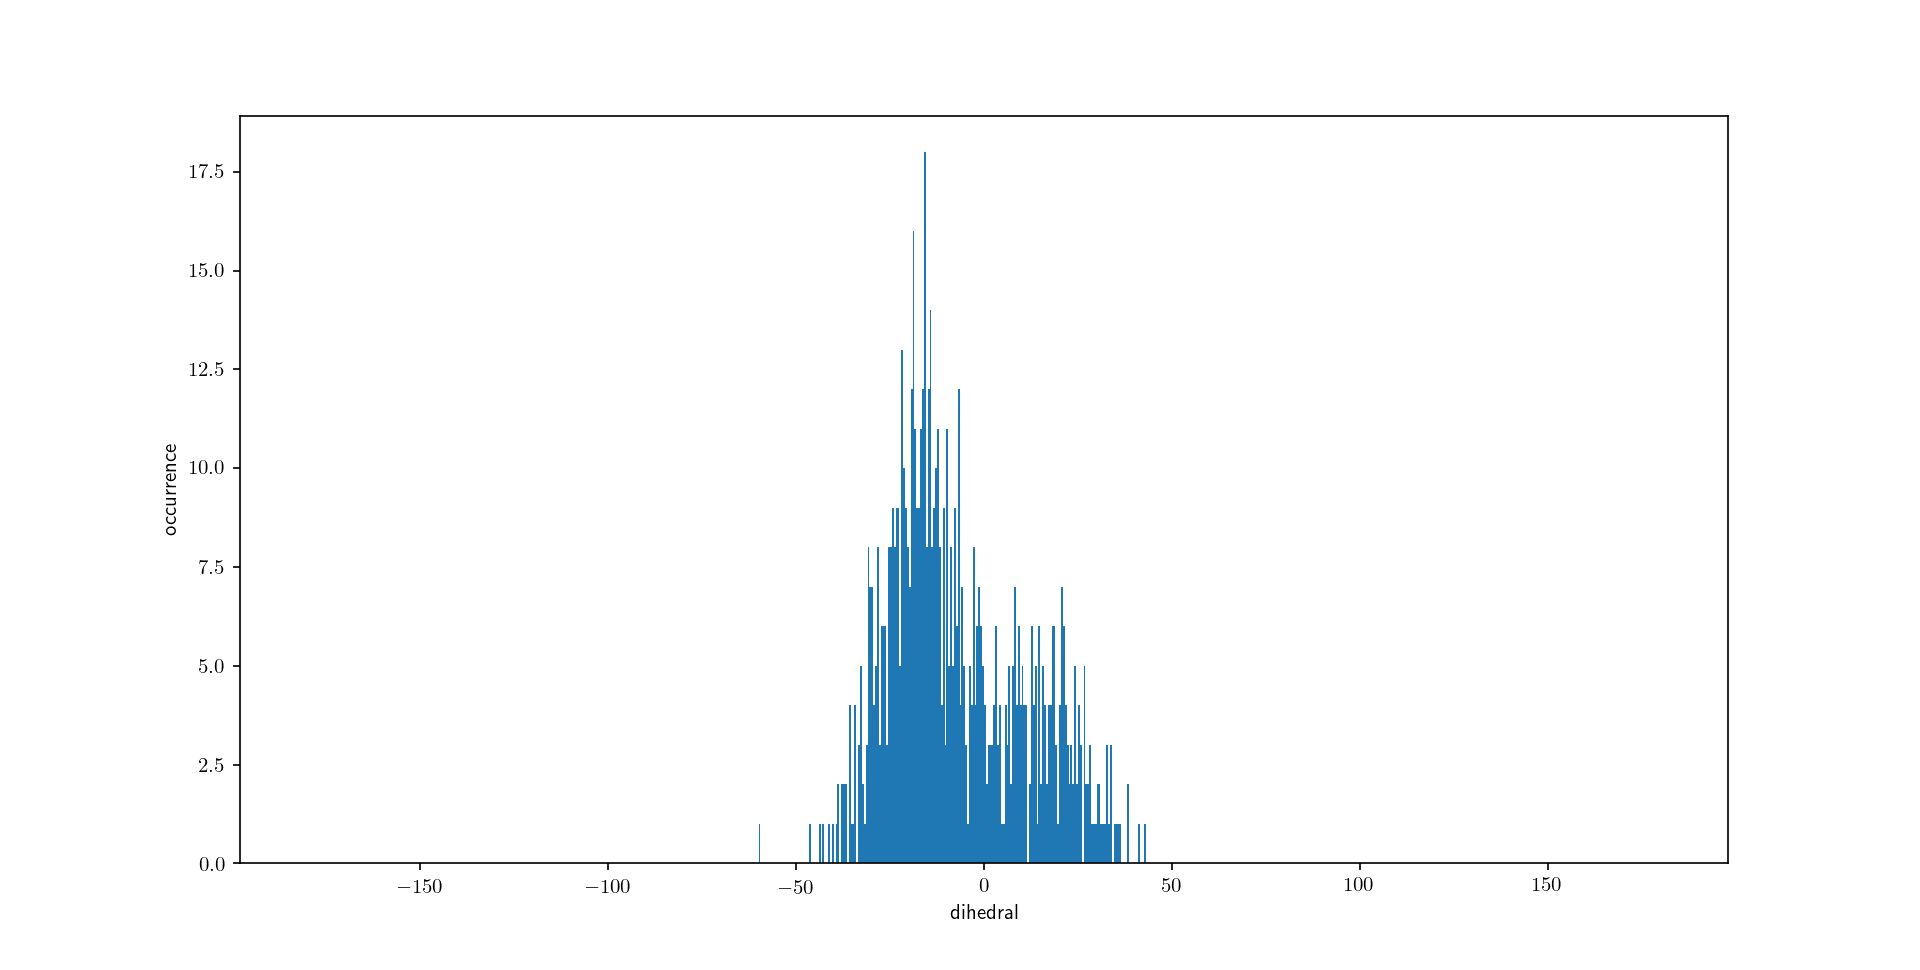
\includegraphics[width=0.95\textwidth]{./figures/dih49_distrib.png}
\caption{Distribution of dihedral 49.} 
\label{fig:dih49distrib}
\end{figure}
%%%%%%%%%%%%%%%%%%%%%%%%%%%%%%%%%

This suggests that 2D-correlation is a powerful tool (see Fig. \ref{dihh49dih52}), as it reveals the separation in the distribution of dihedral 49, and that detection could be obtained either via analysis of the multidimensional correlation, or via analysis of the angular displacement, which mantains time information.

The retinal has been averaged both in a ``naive'' way ignoring this aspect (i.e. authomatic detection of ``oscillating'' dihedrals) and by manually requiring detection of 2 or more clusters for dihedral 49. The former method is denoted via the \textit{descriptor} ``naive''.

Let us now look at the most important geometries.

%%%%%%%%%%%%%%%%%%%%%%%%%%%%%%%%%
% Naive and not major basin
\begin{figure}[H]
\centering
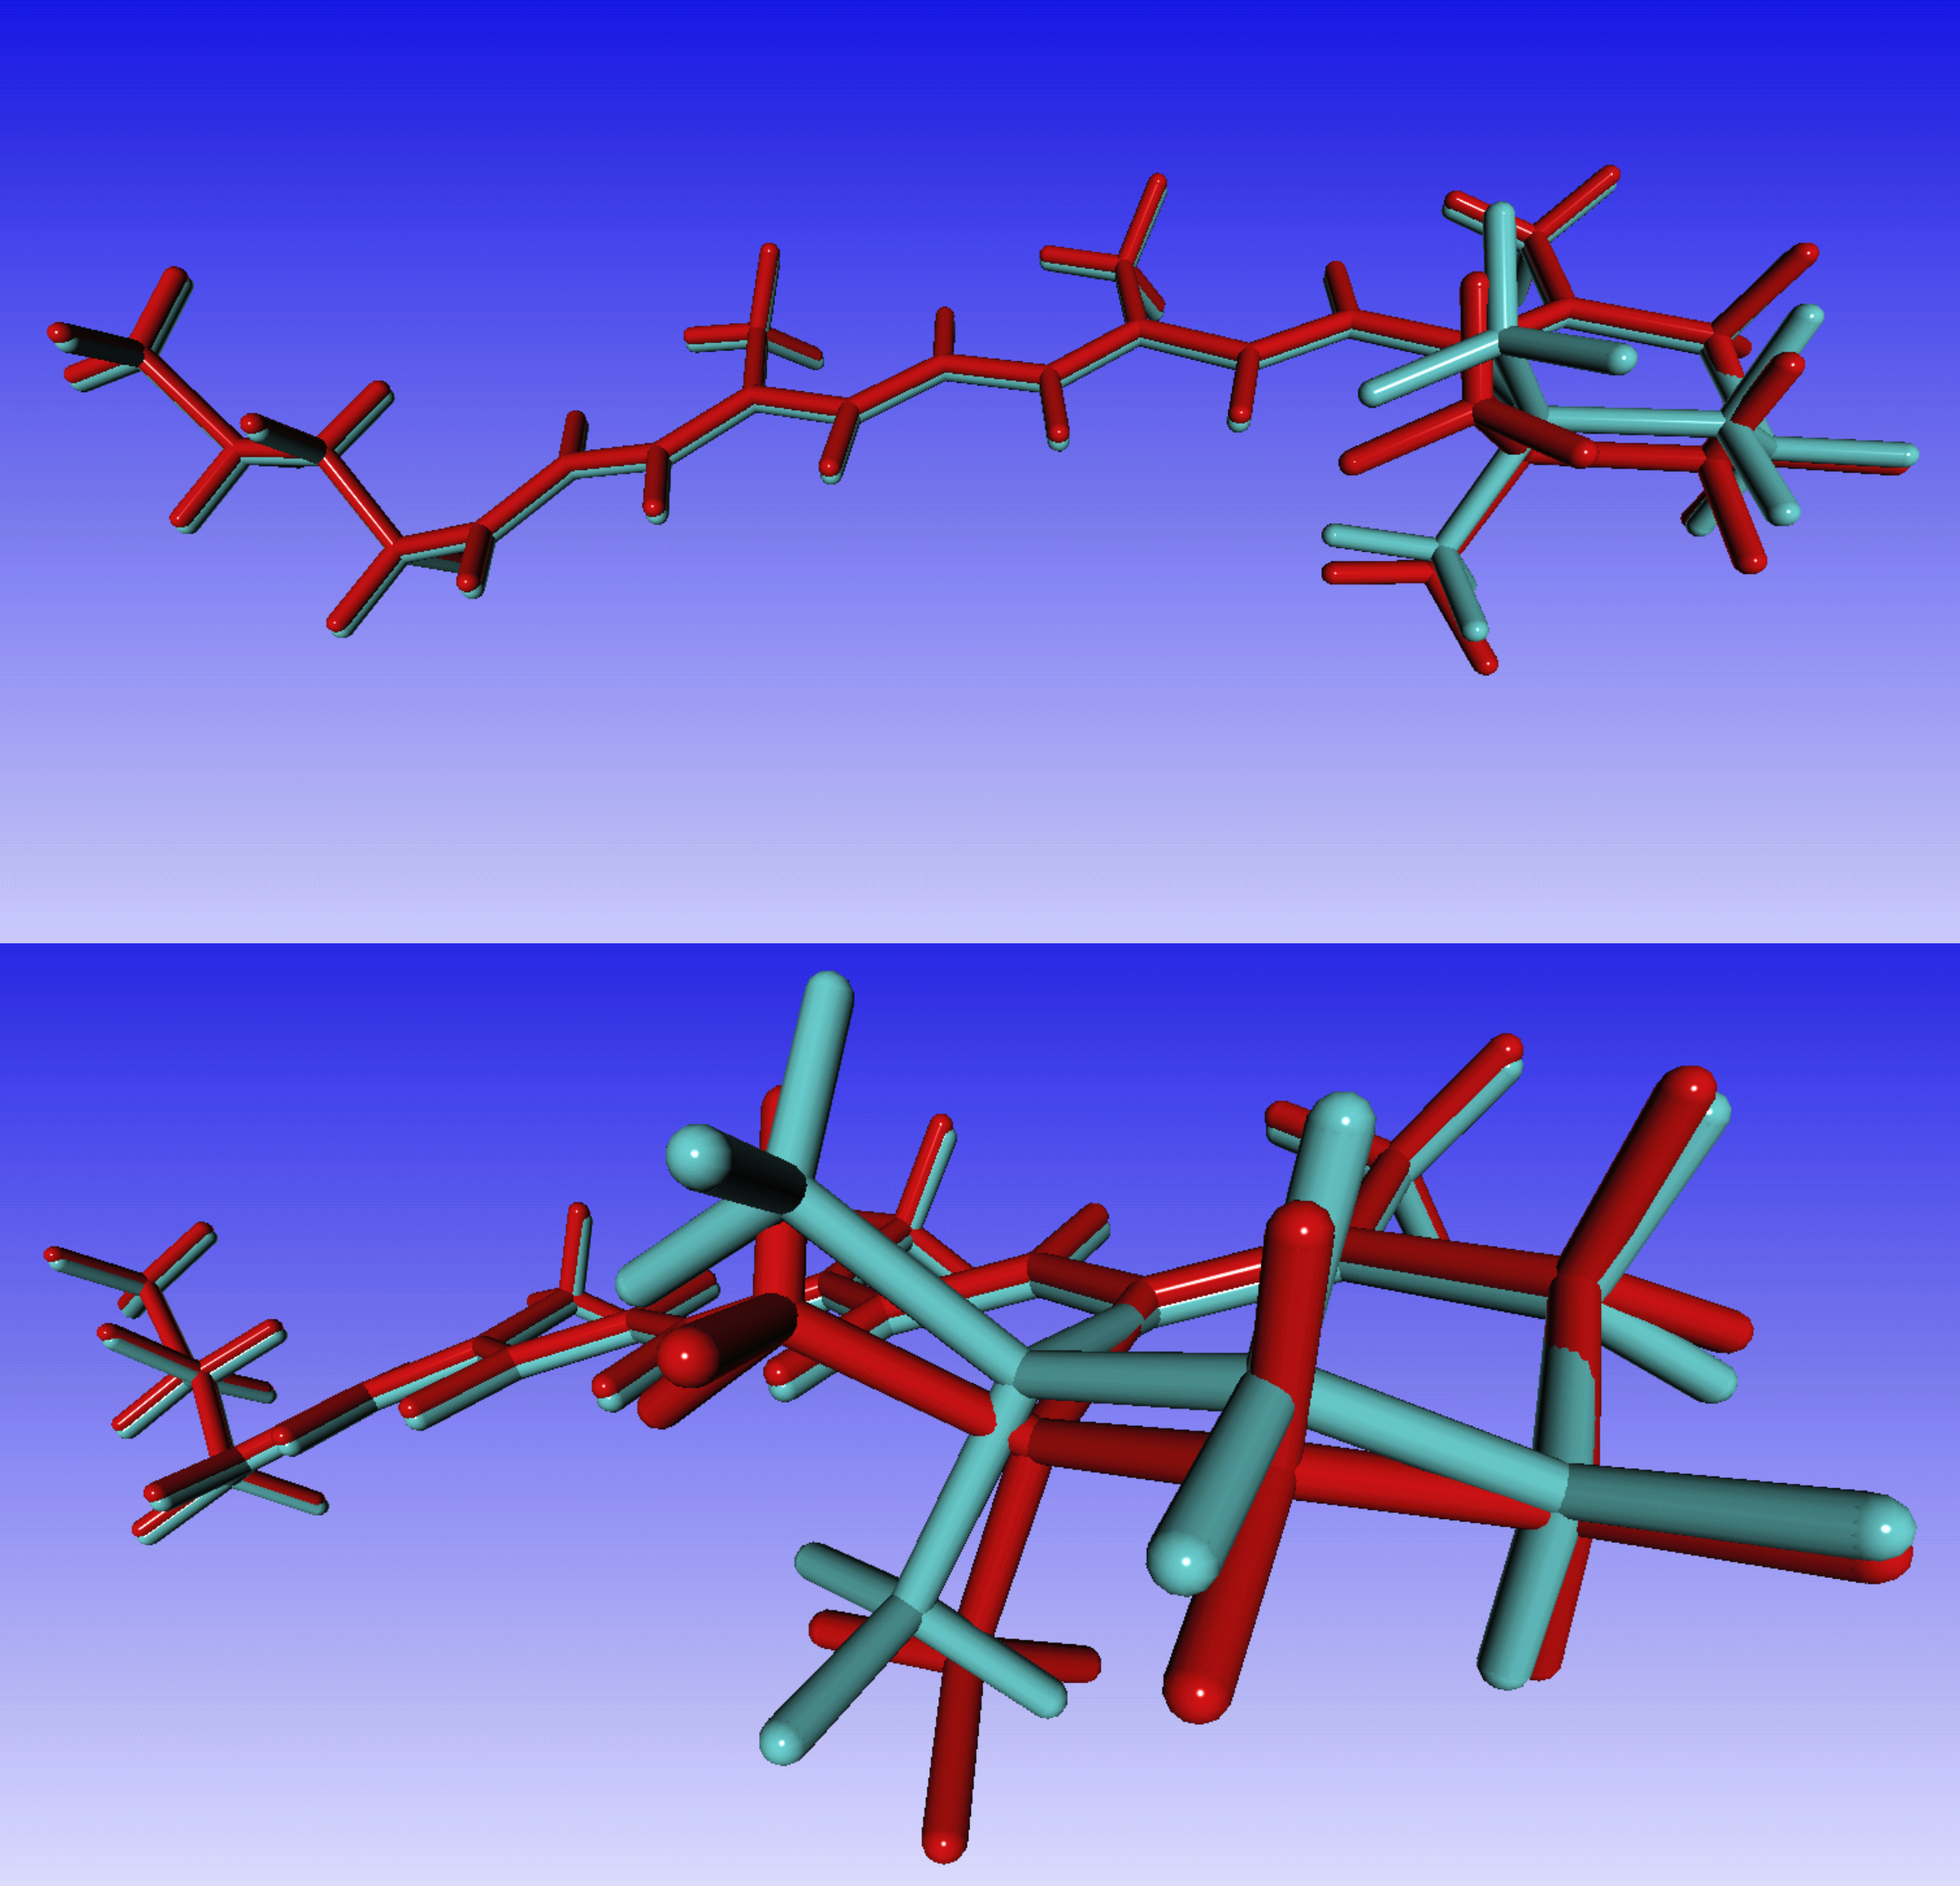
\includegraphics[width=0.95\textwidth]{./figures/mb_comp.png}
\caption{Comparison of averaging within the major basin with (red) and without (white) basin recognition for dihedral 49.} 
\label{fig:mb_comp}
\end{figure}
%%%%%%%%%%%%%%%%%%%%%%%%%%%%%%%%%

%%%%%%%%%%%%%%%%%%%%%%%%%%%%%%%%%
% Naive and not minor basin
\begin{figure}[H]
\centering
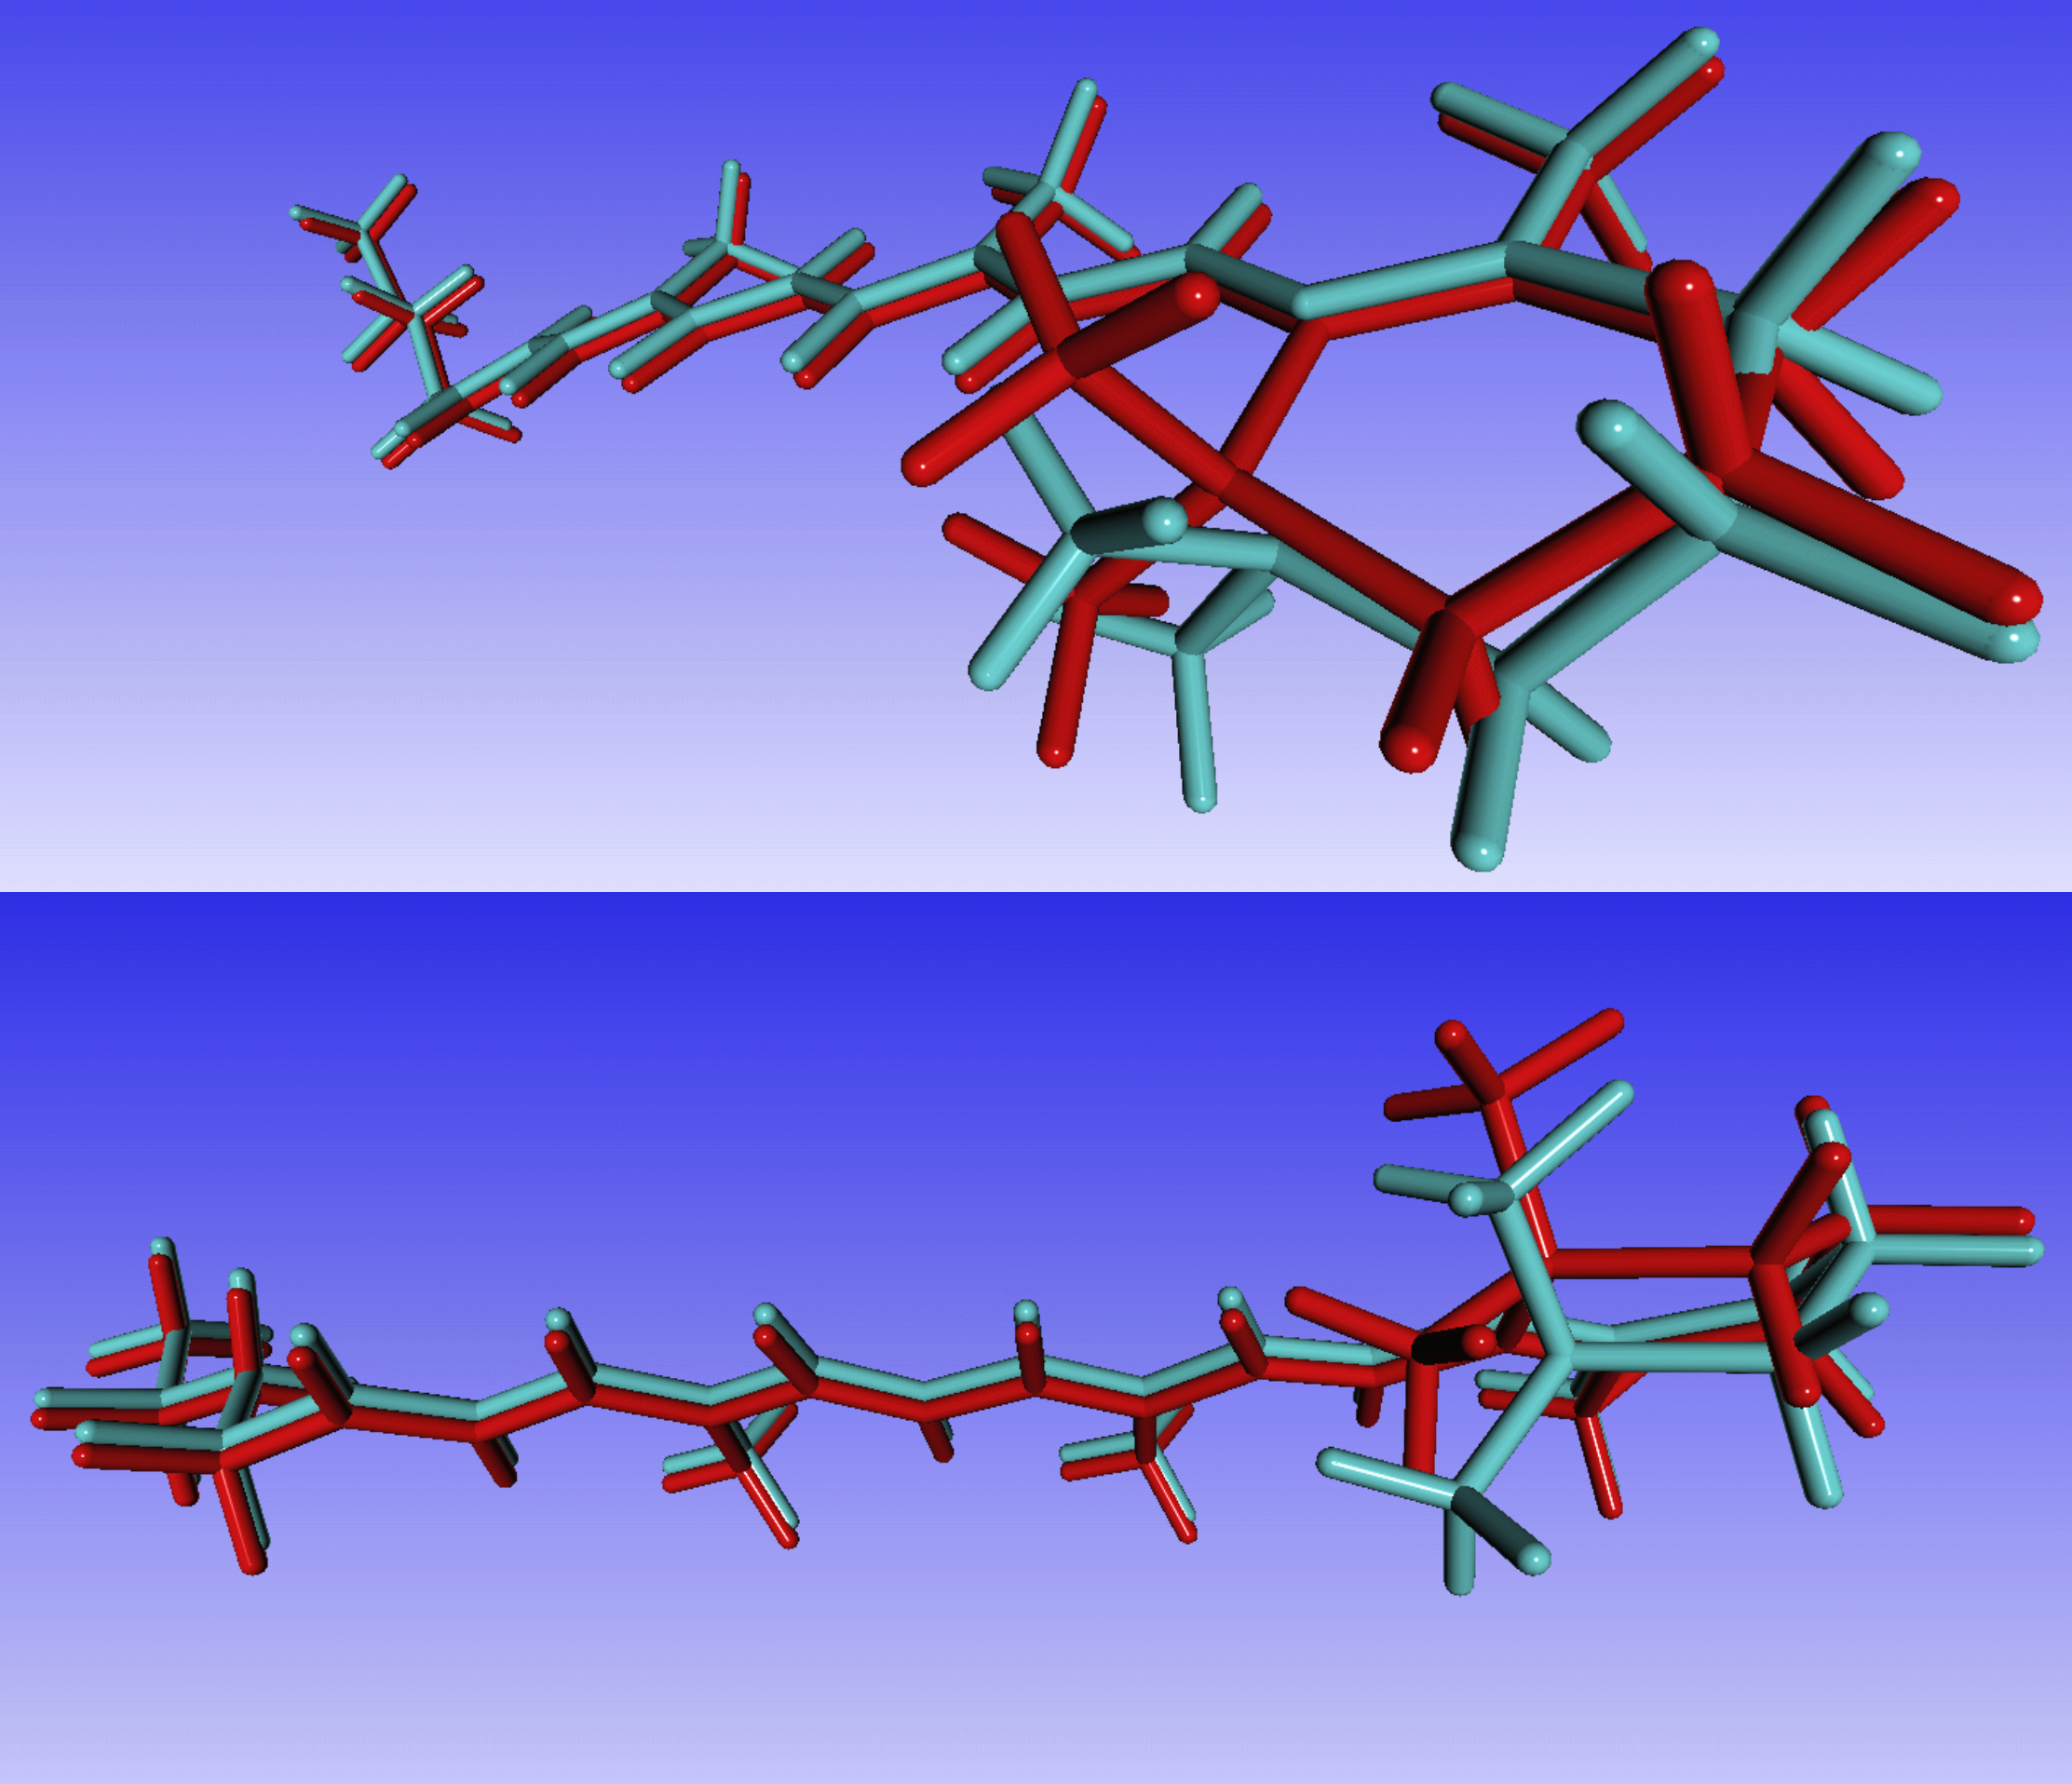
\includegraphics[width=0.95\textwidth]{./figures/minb_comp.png}
\caption{Comparison of averaging within the minor basin with (red) and without (white) basin recognition for dihedral 49.} 
\label{fig:minb_comp}
\end{figure}
%%%%%%%%%%%%%%%%%%%%%%%%%%%%%%%%%
Geometrically speking, the cluster recognition on dihedral 49 does not cause great changes, but these ``propagate'' slighlty to the atoms connected to it. (see Fig. \ref{fig:mb_comp} and Fig. \ref{fig_minb_comp}).

Clearly selecting the major or minor basin corresponds to the two envelope-like configurations of the polysubsituted cyclohexene (see Fig \ref{}).

%%%%%%%%%%%%%%%%%%%%%%%%%%%%%%%%%
% Major vs minor basin
\begin{figure}[H]
\centering
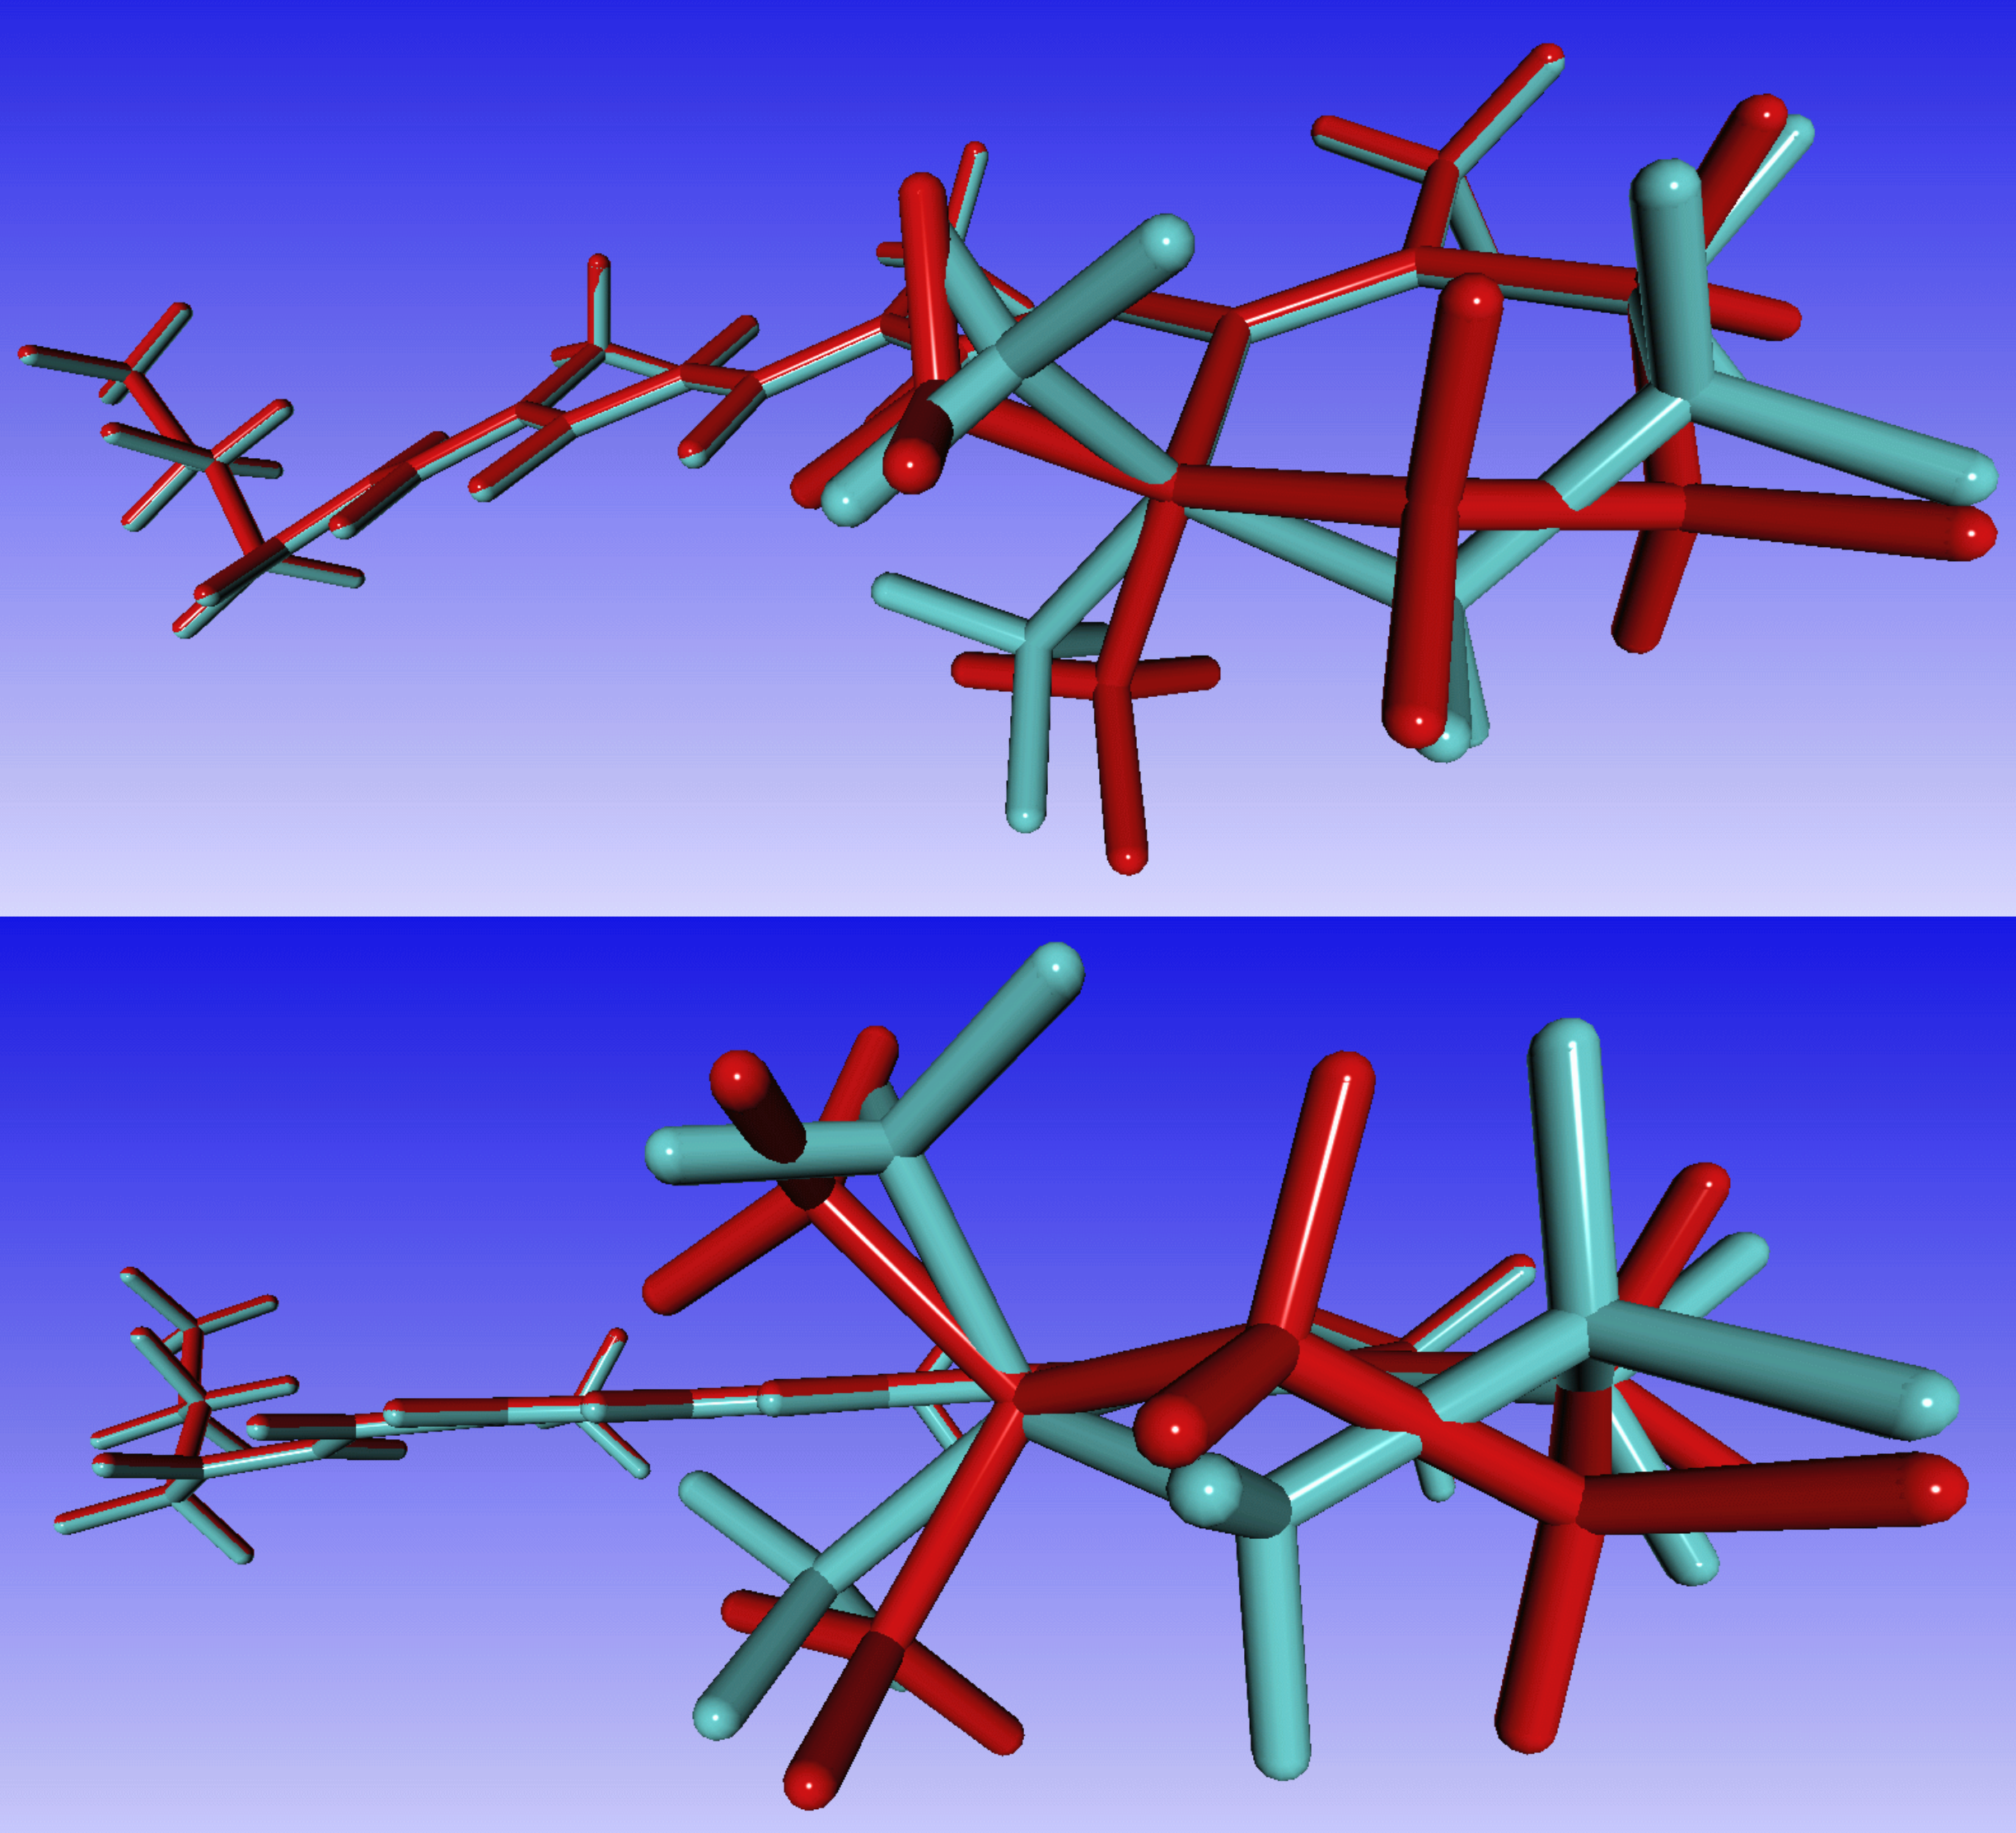
\includegraphics[width=0.95\textwidth]{./figures/mb_minb_comp.png}
\caption{Comparison of averaging within the major(red) and minor(white) basin. Dihedral 49 is averaged in the specific basin.} 
\label{fig:dih49dih52}
\end{figure}
%%%%%%%%%%%%%%%%%%%%%%%%%%%%%%%%%

%%%%%%%%%%%%%%%%%%%%%%%%%%%%
% Excitation energy table 
\begin{table}[h]
\footnotesize
\centering
\caption{Excitation energies and ground state energy for different averaged geometries. The ground state energy is calculated from the most stable frame in the trajectory. mb = major basin, minb = minor basin, pf = pick first, none = straightforward averaging}
\label{tab:ex_ret_avrg}
\begin{tabular}{lcc}
& \textbf{$\varepsilon_\mathrm{gas}$ / eV} & \textbf{$\Delta E_{GS}$ / Kcal/mol}  \\ 
\textbf{mb-mb-naive} & 3.141 & 1.89\\ 
\textbf{mb-mb} & 3.138 & 1.34\\
\textbf{minb-mb-naive} & NA & NA \\
\textbf{minb-mb} & 3.137 & 1.60\\
\textbf{mb-pf} & 3.060 & \\ 
\textbf{none-mb} & 2.810 & 15.630\\ 
\textbf{none-pf} & 2.717 & 15.984\\ 
\textbf{pf-mb} &  3.152 & 3.469\\ 
\textbf{pf-pf} & 3.070 & 3.813\\ 
\textbf{Avg. 750} &  3.044 \\ 
\textbf{Std. Dev. 750} &  0.126\\ 
\end{tabular}
\end{table}
%%%%%%%%%%%%%%%%%%%%%%%%%%

From table \ref{tab:ex_ret_avrg} we can see that:
\begin{itemize}
 \item straightforward averaging of the oscillating dihedrals (ciclohexene) causes a high ground-state energy (~15 Kcal/mol). The excitation energy is affected, but less (0.3-0.4 eV, which is approximately half of 15 Kcal/mol==0.65 eV).
 Also the oscillator strength is affected (~1.8 vs ~2.4 for all other geometries).
 \item as expected, methyls are not that important
 \item the basin-based averaging seems to lead to reasonable groun-state energies and excitation energies
 \item cluster recognition for dihedral 49 did not cause massive changes
\end{itemize}


\subsection{Bond-length-alternation bins}
The bond-length-alternation has been shown to be more important to the excitation energy than the environment. The bins containing frames which correspond to the 6 important basins were given by Suli. These frames were used to evaluate the average excitation energies for both the isolated and embedded retinal. The results are compared to the total-750-frames average values in table \ref{tab:ex_bins}.

We need to check if this are correct for the final trajectory shared because the averages don't seem so different.

%%%%%%%%%%%%%%%%%%%%%%%%%%%%
% Excitation energy table 
\begin{table}[h]
\footnotesize
\centering
\caption{Bond alternation averages in eV.}
\label{tab:ex_bins}
\begin{tabular}{cccc}
& \textbf{$\langle \varepsilon_\mathrm{gas} \rangle$ / eV} & \textbf{$\langle \varepsilon_\mathrm{emb} \rangle$ / eV} & \textbf{$\delta \varepsilon$ / eV}  \\ 
\textbf{Bin 1} & 2.989 & 3.286 & 0.297\\ 
\textbf{Bin 2} & 3.043 & 3.415 & 0.372\\ 
\textbf{Bin 3} & 3.044 & 3.418 & 0.374\\ 
\textbf{Bin 4} & 3.040 & 3.412 & 0.372\\ 
\textbf{Bin 5} & 3.055 & 3.438 & 0.383\\ 
\textbf{Bin 6} & 3.136 & 3.486 & 0.350\\ 
\textbf{Avg. 750} &  3.044 & 3.418 & 0.374\\ 
\textbf{Std. Dev. 750} &  0.126 & 0.183 &\\ 
\end{tabular}
\end{table}
%%%%%%%%%%%%%%%%%%%%%%%%%%


%%%%%%%%%%%%%%%%
% Bibliography %
%%%%%%%%%%%%%%%%
\clearpage
%\bibliography{references}
\bibliographystyle{achemso}

\end{document}





































